\section{Initial Experiments}

We start with finding the ranking for nodes recommended in an existing network. We consider a synthetic network $G(N,m,f,h)$ with parameters $N=1000, m=2, f=0.2$ as fixed parameters, and $h$ being varied from [0.0, 1.0], step-size=0.1.

We show in figure \ref{fig-hom} the initial structure of the network along with degree distribution and degree growth for the network, which is grown considering only preferential-attachment and homophily as in equation \ref{pref-hom}. We find our results similar to \cite{karimi2018homophily}, showing similar network characteristics.

\begin{figure}[hbt!]
	\centering
	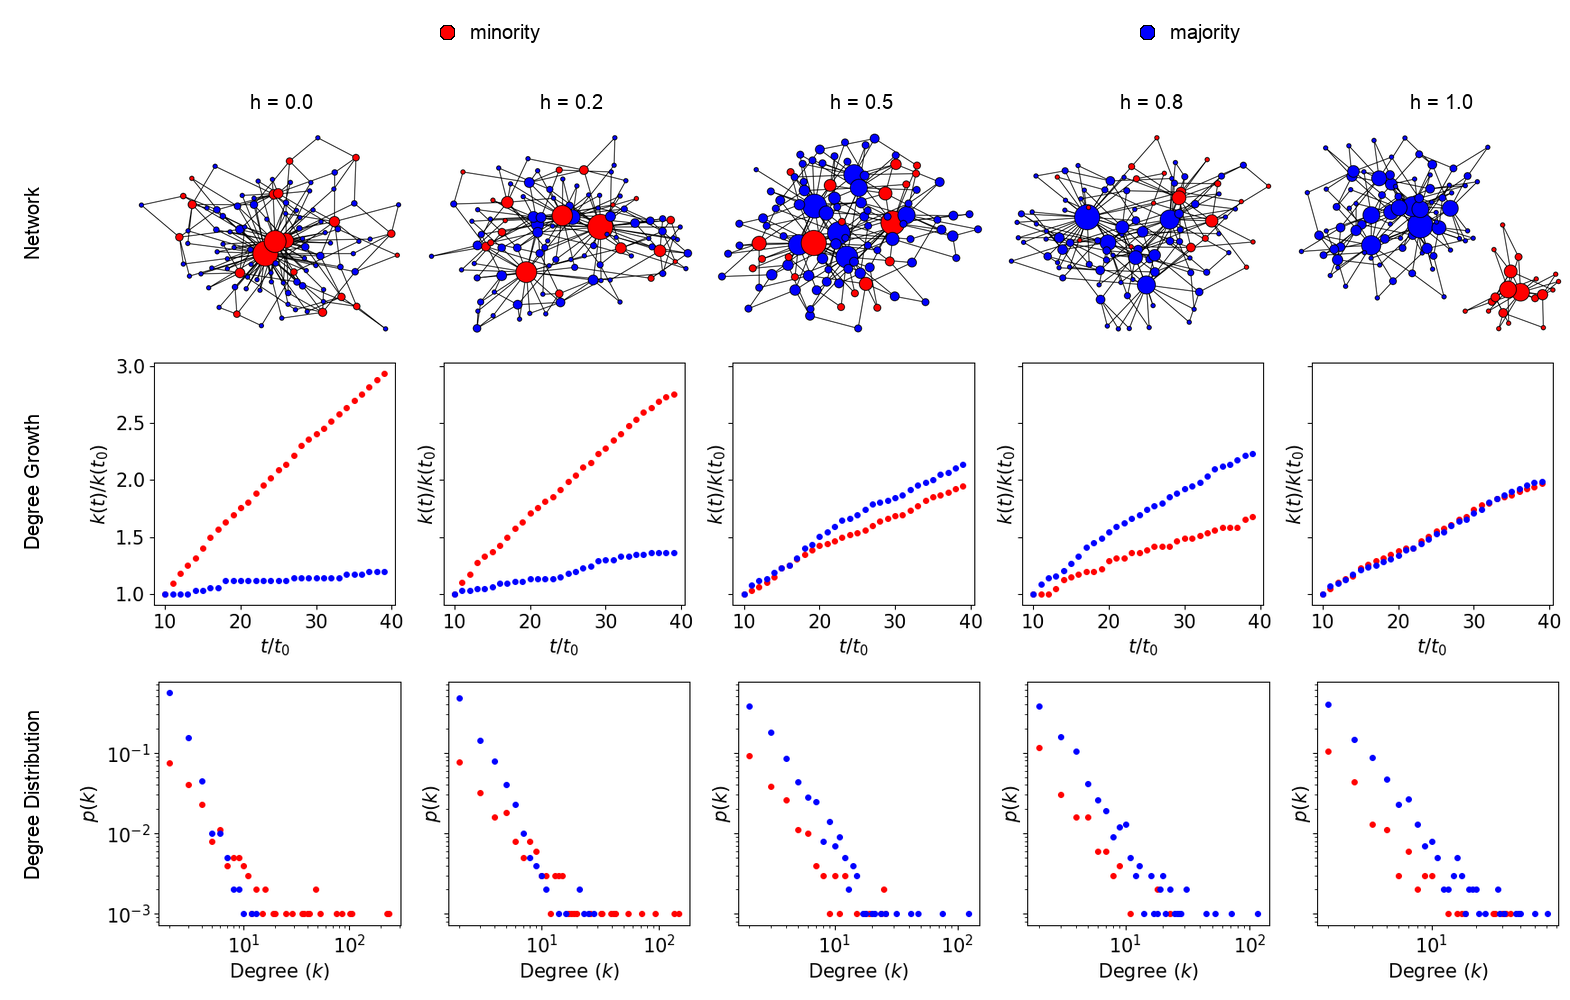
\includegraphics[scale=0.23]{images/proposal_figure_1}
	\caption{Network grown using preferential-attachment and homophily. The minority fraction has been set fixed to 0.2, number of edges added per iteration is 2. The homophily parameter ranges from 0.0(complete heterophily) to 1.0(complete homophily). Tile A shows a visualization of the network with 100 nodes, for different homophily parameters. For Tile B and C, the network contains 1000 nodes, averaged over 5 iterations.}
	\label{fig-hom}
\end{figure}

\begin{figure}
	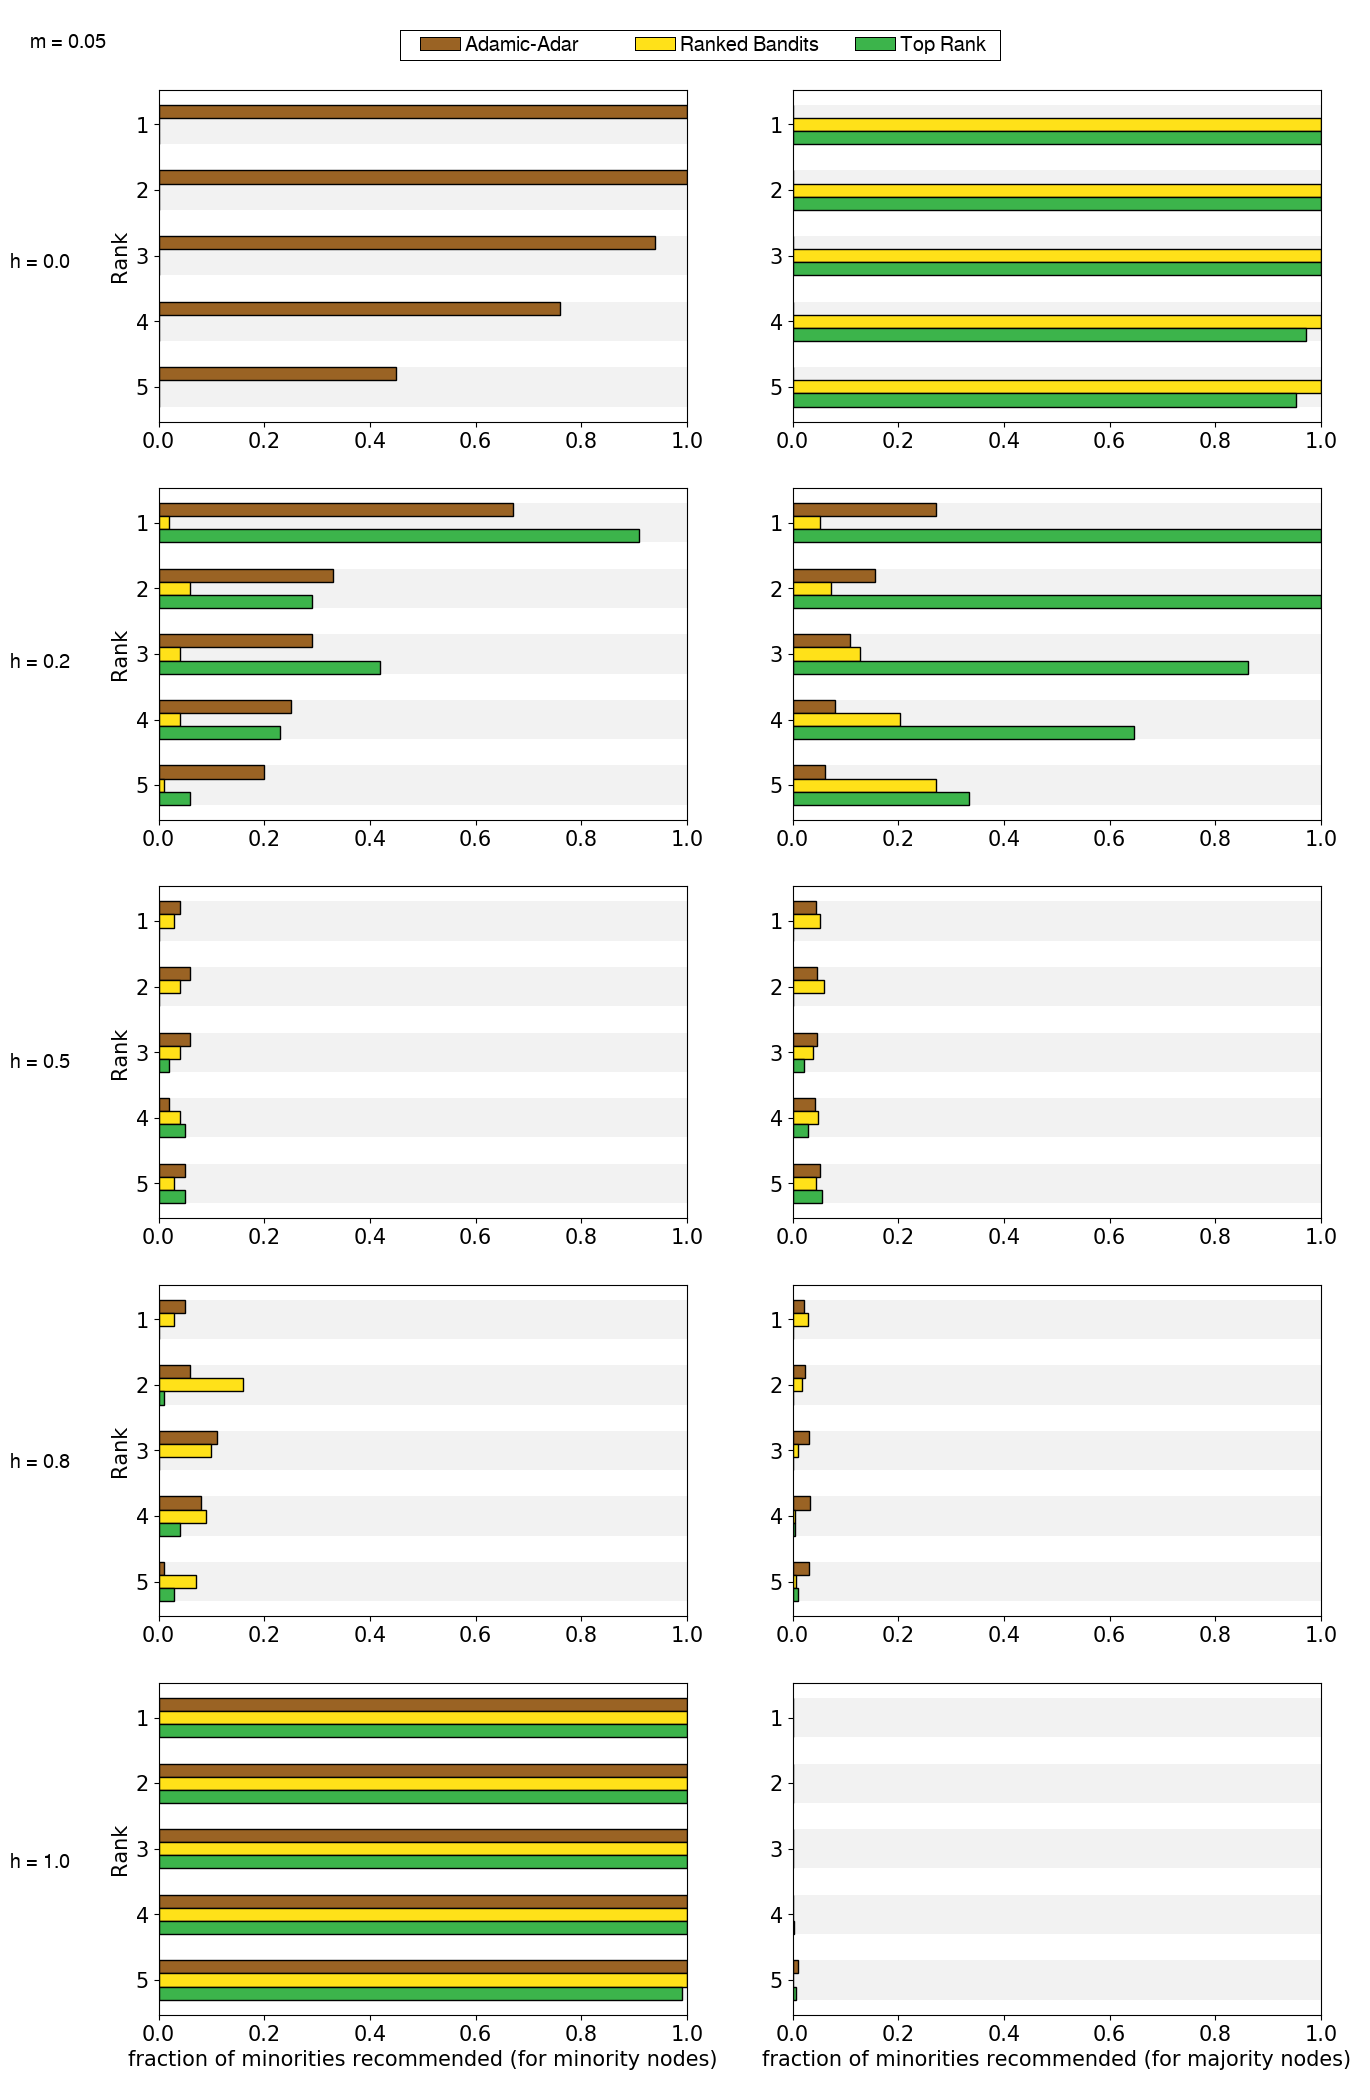
\includegraphics[scale=0.28]{images/proposal_figure_3_1}
	\caption{Fraction of minorities recommended in the top 5 ranks for the two node groups. On the left hand side is the recommendation provided to minority nodes, while on the right-hand side are the recommendations provided to majority nodes. The 3 different ranking schemes are shown with three colors. The network considered has 1000 nodes, with a minority fraction of 0.05.}
	\label{fig-rank_1}
\end{figure}

\begin{figure}
	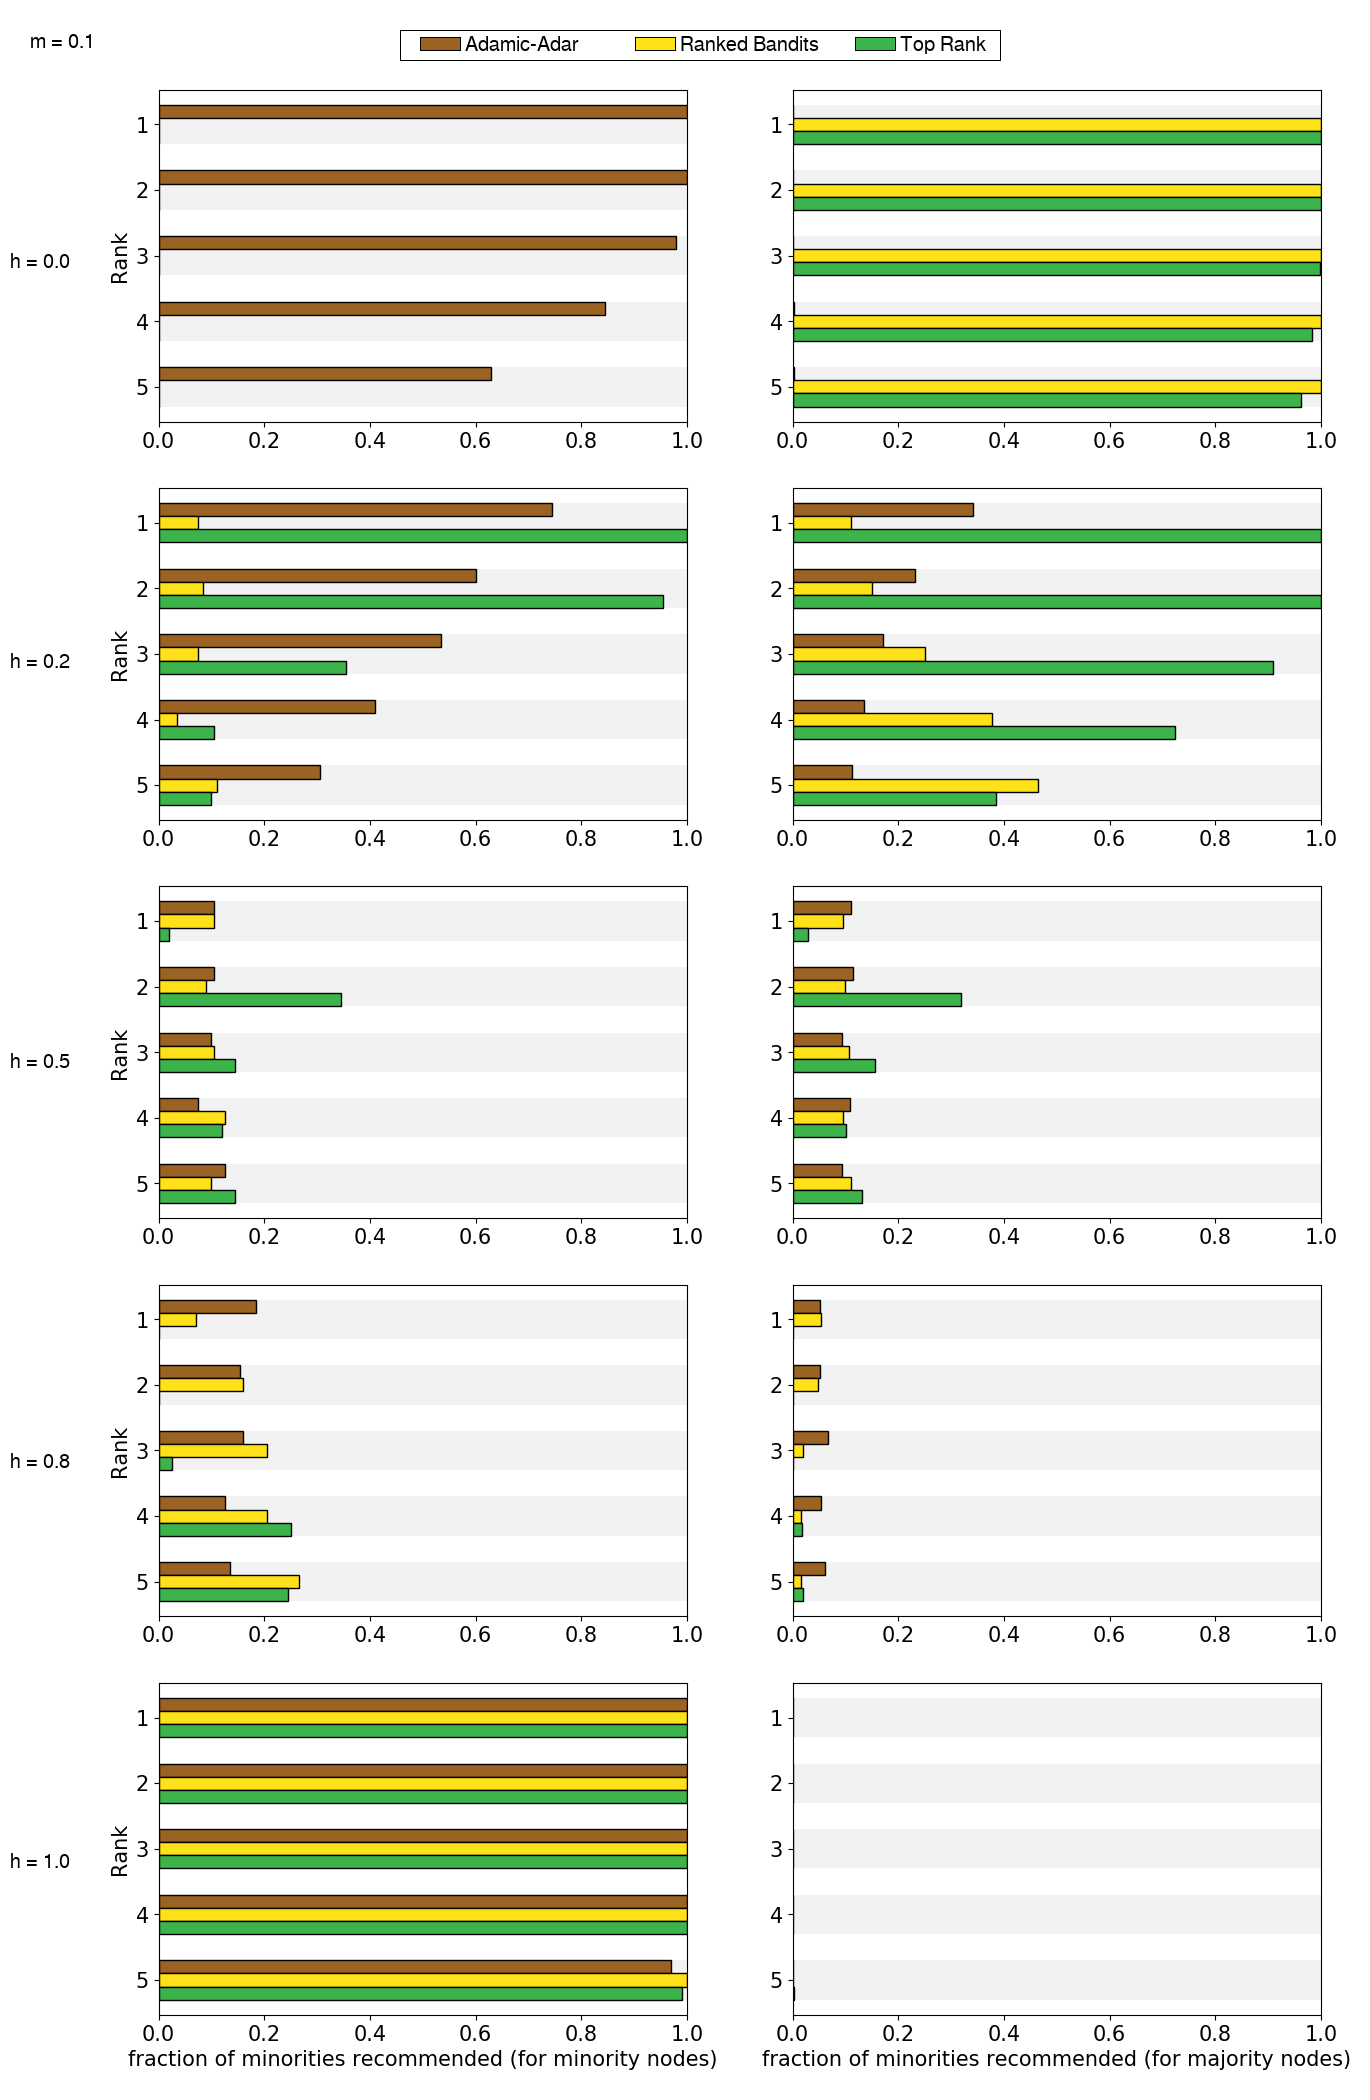
\includegraphics[scale=0.28]{images/proposal_figure_3_2}
	\caption{Fraction of minorities recommended in the top 5 ranks for the two node groups. On the left hand side is the recommendation provided to minority nodes, while on the right-hand side are the recommendations provided to majority nodes. The 3 different ranking schemes are shown with three colors. The network considered has 1000 nodes, with a minority fraction of 0.1.}
	\label{fig-rank_2}
\end{figure}
\begin{figure}
	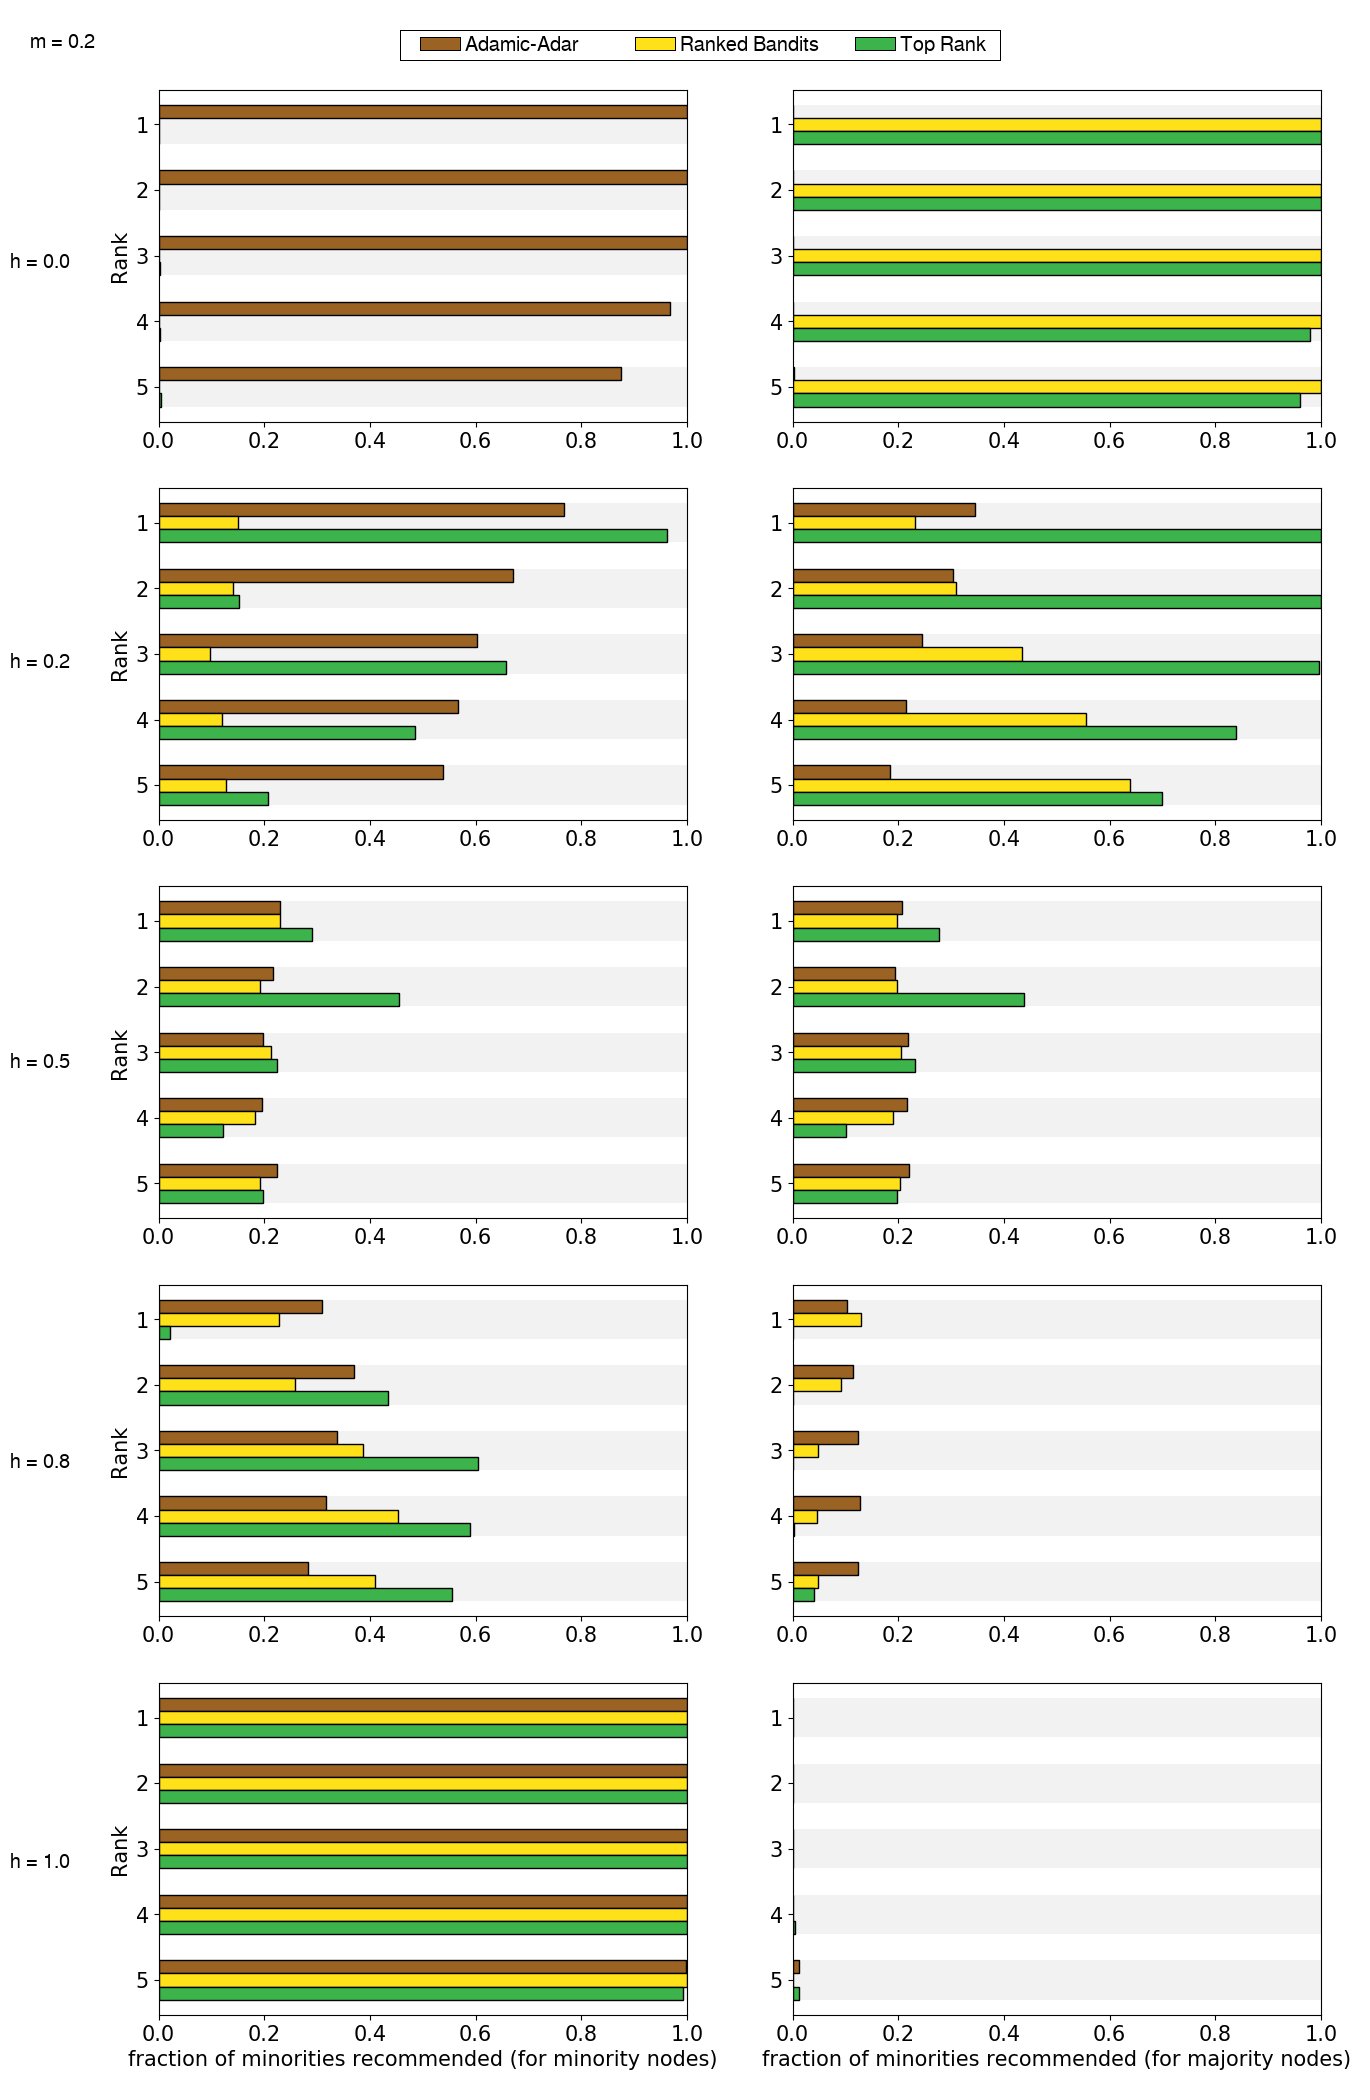
\includegraphics[scale=0.28]{images/proposal_figure_3_3}
	\caption{Fraction of minorities recommended in the top 5 ranks for the two node groups. On the left hand side is the recommendation provided to minority nodes, while on the right-hand side are the recommendations provided to majority nodes. The 3 different ranking schemes are shown with three colors. The network considered has 1000 nodes, with a minority fraction of 0.2.}
	\label{fig-rank_3}
\end{figure}
\begin{figure}
	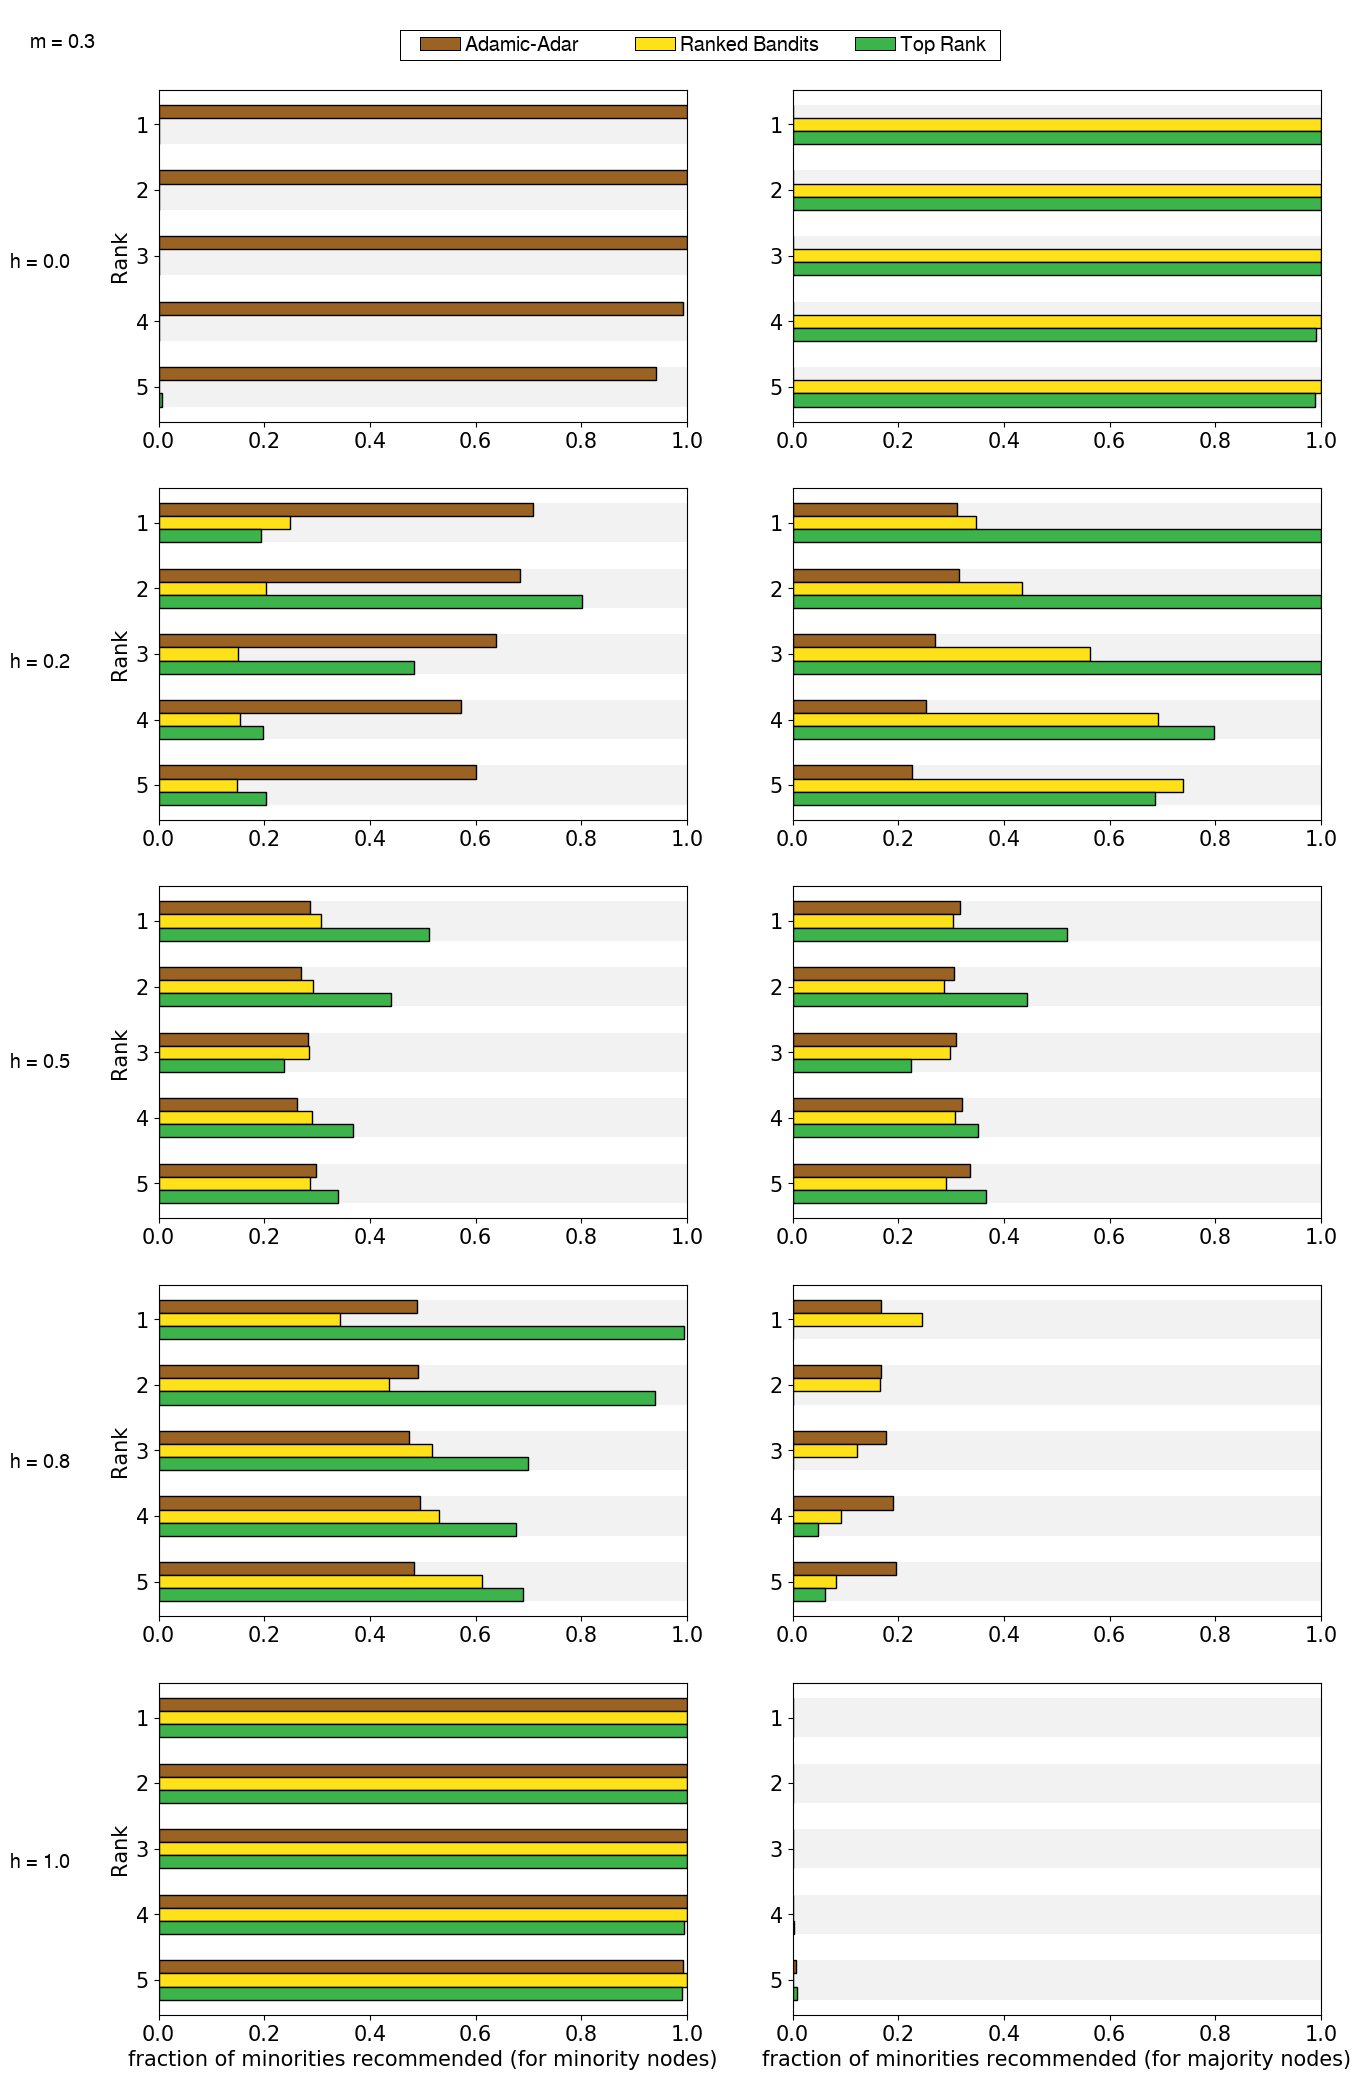
\includegraphics[scale=0.28]{images/proposal_figure_3_4}
	\caption{Fraction of minorities recommended in the top 5 ranks for the two node groups. On the left hand side is the recommendation provided to minority nodes, while on the right-hand side are the recommendations provided to majority nodes. The 3 different ranking schemes are shown with three colors. The network considered has 1000 nodes, with a minority fraction of 0.3.}
	\label{fig-rank_4}
\end{figure}
\begin{figure}
	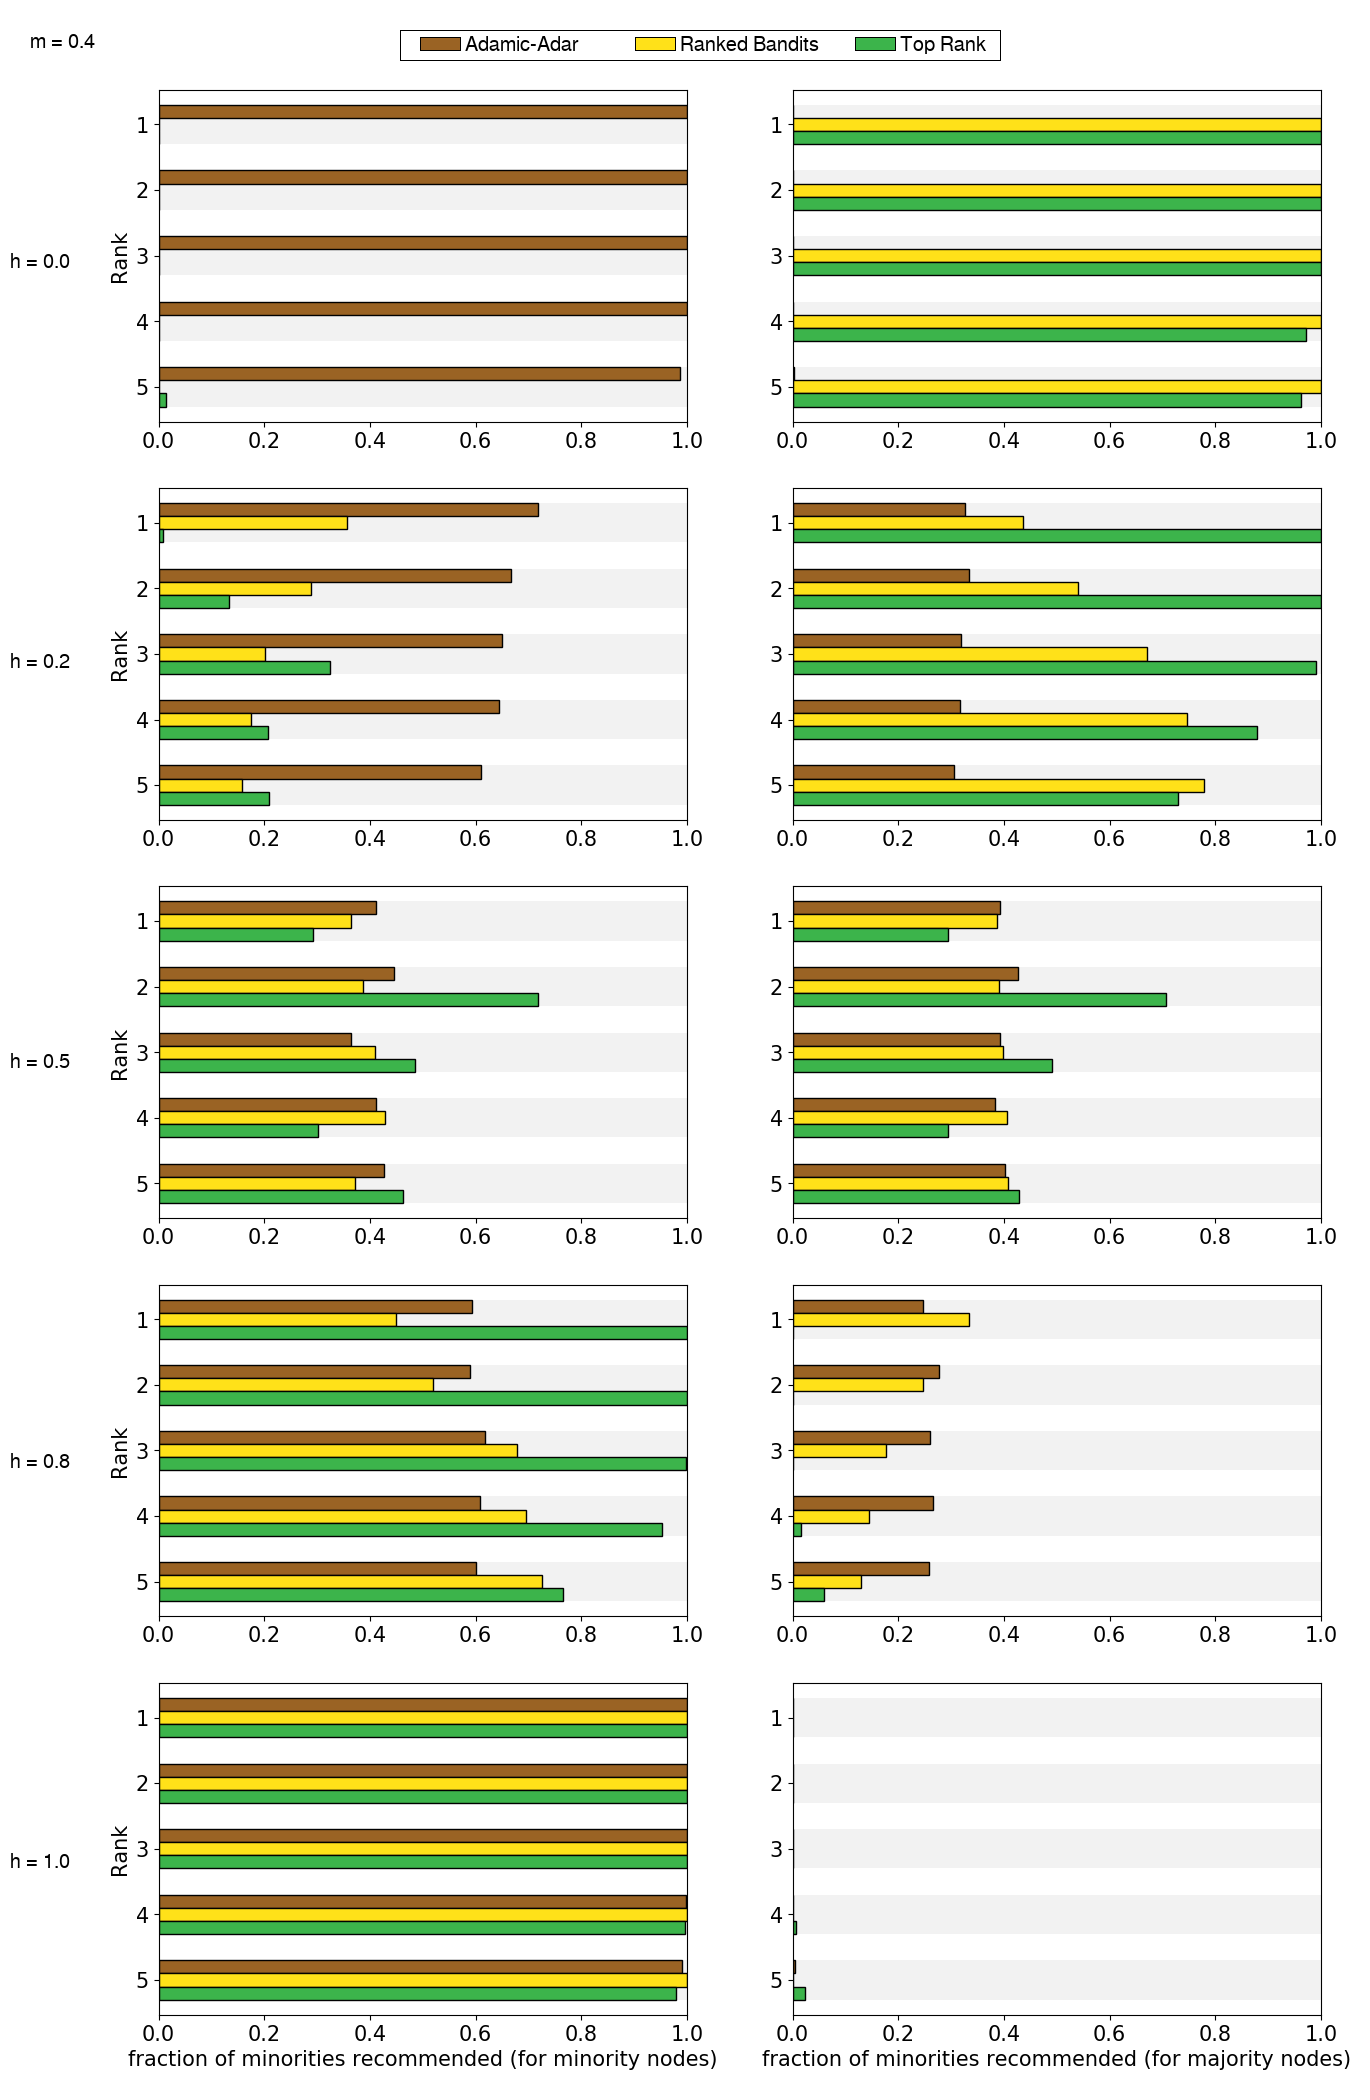
\includegraphics[scale=0.28]{images/proposal_figure_3_5}
	\caption{Fraction of minorities recommended in the top 5 ranks for the two node groups. On the left hand side is the recommendation provided to minority nodes, while on the right-hand side are the recommendations provided to majority nodes. The 3 different ranking schemes are shown with three colors. The network considered has 1000 nodes, with a minority fraction of 0.4.}
	\label{fig-rank_5}
\end{figure}
\begin{figure}
	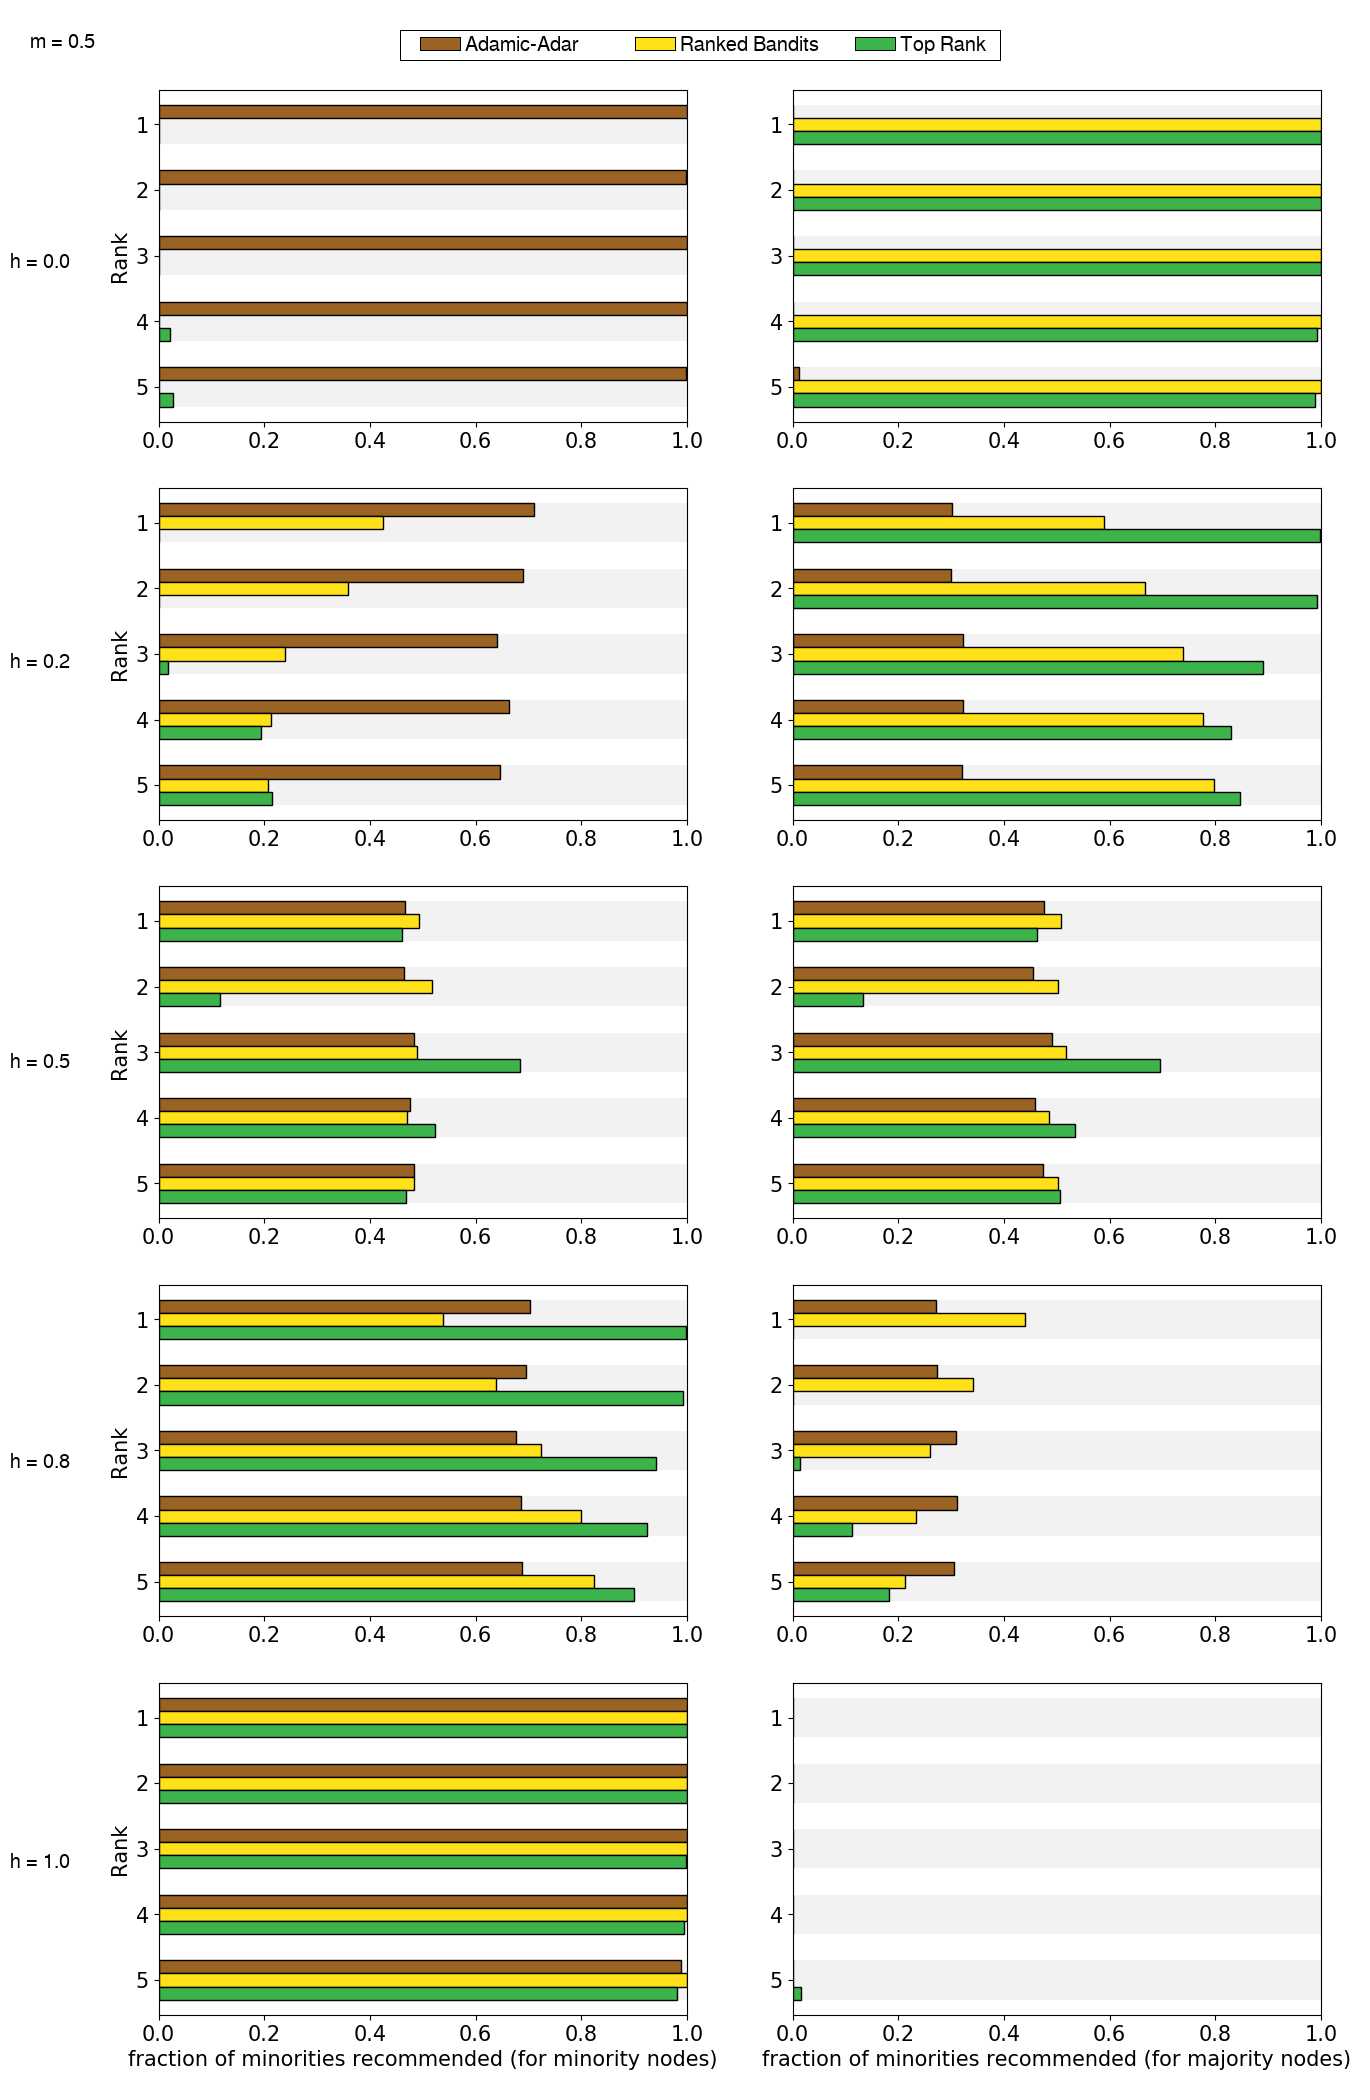
\includegraphics[scale=0.28]{images/proposal_figure_3_6}
	\caption{Fraction of minorities recommended in the top 5 ranks for the two node groups. On the left hand side is the recommendation provided to minority nodes, while on the right-hand side are the recommendations provided to majority nodes. The 3 different ranking schemes are shown with three colors. The network considered has 1000 nodes, with a minority fraction of 0.5.}
	\label{fig-rank_6}
\end{figure}

For the network, with varying homophily, we run our Multi-Armed Bandits approach of ranking for all the nodes as devised in \cite{radlinski2008learning}. We take the number of slots to be 5, thus training for 5 ranking spots per node in the network. The underlying MAB algorithm being used is $\epsilon$-Greedy (with $\epsilon=0.1$). We use the sample-average method for estimating the best action values, where actions are basically the choice of nodes among the network to recommend. The reward function returns 1, when the node recommended is chosen by our clicking model, and a reward value of 0 if the node recommended is not chosen. Details about the node choice model is provided in the Methods section. We train our recommender system for $10^5$ iterations. We then see at which position nodes are ranked, based on the node group asking for recommendation. We also run the TopRank algorithm \cite{lattimore2018toprank} and the Adamic-Adar Index to compare our results. Figure \ref{fig-rank_1} - Figure \ref{fig-rank_6} shows our results for different minority groups.

For the complete hetrophilic case, a sharp difference can be seen in the Adamic-Adar ranking and the Ranked-Bandits ranking. This is evident since the Adamic-Adar Index does not consider the homophily value for making link predictions, since the minority nodes have majority nodes as their neighbours always and they in turn have only minority neighbours, other minority nodes are recommended minority nodes. The Ranked-Bandit however considers the homophily parameter and hence the recommendations are more aligned to the idea of homophily.

\bigskip